\section{Evaluation}
\label{sec:evaluation}

We evaluate CLIO along three axes: (1)~agentic efficiency, whether CLIO
reduces LLM token consumption and latency compared to raw catalog access;
(2)~science-aware accuracy, whether dimensional conversion and formula
normalization improve retrieval precision where text-based methods fail;
and (3)~storage integration and scaling, whether CLIO can serve as the
search layer for IOWarp's tiered blob storage and scale across
distributed HPC nodes.

\subsection{Experimental Setup}
\label{sec:setup}

\textbf{Platforms.} Single-node experiments run on Linux 6.17 with
Python 3.11, DuckDB 1.1, and all-MiniLM-L6-v2 embeddings (384-dim).
Distributed experiments run on NCSA DeltaAI using NVIDIA GH200 Grace
Hopper nodes (72~ARM Neoverse V2 cores, 480\,GB unified CPU+GPU
memory, NVLink-C2C, Slingshot-11) with a 2.5M arXiv abstract corpus
across 4~DuckDB shards. IOWarp experiments run inside Docker with the
\texttt{iowarp/deps-cpu} image and Chimaera runtime v1.0.3.

\textbf{Controlled benchmark.} 210 synthetic documents across seven
scientific domains (Table~\ref{tab:dataset}) with deliberate unit
heterogeneity: each document contains known numeric-unit pairs, and
the same physical quantities are expressed in different SI prefixes
across documents. Ground truth is generated programmatically: a
document is relevant to a query if and only if it contains a
measurement within the query's numeric range after SI conversion.
80~queries test cross-unit, same-unit, formula, and multi-constraint
retrieval. We additionally validate on 288 real NOAA observatory
documents~\cite{ghcn2012} to assess ecological validity.

\begin{table}[!t]
\centering
\caption{Benchmark corpus: 210 documents, 80 queries across seven domains.}
\label{tab:dataset}
\small
\renewcommand{\arraystretch}{1.15}
\begin{tabular}{@{}l r l@{}}
\toprule
\textbf{Domain} & \textbf{Docs} & \textbf{Key Measurements} \\
\midrule
Materials science   & 40 & MPa, kPa, mm, g, mg \\
\rowcolor{gray!5}
Atmospheric science & 40 & Pa, kPa, hPa$^\dagger$, m/s, km/h \\
Fluid dynamics      & 40 & kPa, Pa, MPa, m/s, mm, m \\
\rowcolor{gray!5}
Chemistry           & 30 & s, min, h, mg, g, kg + formulas \\
HPC simulation      & 30 & kPa, Pa, s, mm, m \\
\rowcolor{gray!5}
Cross-domain mixed  & 20 & Multiple domains per doc \\
Negative controls   & 10 & No extractable measurements \\
\midrule
\multicolumn{3}{@{}l}{\textbf{Queries:} 40 cross-unit, 20 same-unit, 10 formula, 10 multi} \\
\bottomrule
\multicolumn{3}{@{}l}{\scriptsize $^\dagger$hPa was unsupported during benchmark construction; now in the registry. No benchmark query targets hPa.}
\end{tabular}
\renewcommand{\arraystretch}{1.15}
\end{table}

\textbf{Baselines.} BM25-only (DuckDB full-text search); Dense-only
(all-MiniLM-L6-v2, cosine similarity); Hybrid BM25+Dense (linear
fusion); String normalization~\cite{numbersmatter2024}; and CLIO's
full pipeline.

\textbf{Metrics.} P@$K$, R@$K$, MRR at $K{=}5$ for retrieval accuracy.
Total tokens (including sub-agent tokens) and wall time for agentic
efficiency.

%% =====================================================================
\subsection{Agentic Efficiency}
\label{sec:agentic-efficiency}

We run 10~scientific discovery queries through three paths using
\texttt{claude-sonnet-4-20250514} and the National Data Platform (NDP)
catalog: (1)~a \textbf{Claude Native Agent} with no domain tools (uses
web search and sub-agents), (2)~an agent with \textbf{NDP-MCP} catalog
access, and (3)~an agent backed by \textbf{CLIO Search}, which indexes
341~NDP datasets into DuckDB and returns ranked citations.

\begin{table}[t]
\centering
\caption{Agentic efficiency on 10~scientific data discovery queries.
All paths use \texttt{claude-sonnet-4-20250514} and the same NDP
catalog. $\Delta$~is relative to the Claude Native Agent.}
\label{tab:l1-results}
\footnotesize
\setlength{\tabcolsep}{4pt}
\renewcommand{\arraystretch}{1.2}
\begin{tabular}{@{}l r r r c@{}}
\toprule
\textbf{Method} & \textbf{Tokens} & \textbf{Tok.\ $\Delta$} & \textbf{Time $\Delta$} & \textbf{Ans.} \\
\midrule
Claude Native Agent & 989{,}417 & ---       & ---       & 10/10 \\
\rowcolor{gray!5}
NDP-MCP             & 988{,}954 & $-$0.05\% & $-$65.68\% & 10/10 \\
\rowcolor{gray!15}
\textbf{CLIO}       & \textbf{474{,}101} & \textbf{$-$52.08\%} & \textbf{$-$91.27\%} & \textbf{10/10} \\
\bottomrule
\end{tabular}
\renewcommand{\arraystretch}{1.15}
\end{table}

CLIO reduces tokens by \textbf{52.08\%} and wall time by
\textbf{91.27\%} (Table~\ref{tab:l1-results}). The native agent and
NDP-MCP consume $\sim$989K tokens through different mechanisms: the
native agent spawns 9~sub-agents (563K main + 426K sub-agent tokens);
NDP-MCP injects raw catalog JSON (989K main tokens). CLIO avoids both
by indexing catalog content locally and returning $\sim$2K tokens of
ranked citations per query (Fig.~\ref{fig:l1-three-path}).
Corpus profiling, branch selection, unit conversion, and result ranking
all execute locally as deterministic operations, leaving the agent to
focus on interpreting results rather than navigating raw data.
CLIO resolves 9 of 10~queries in a single search invocation; one
multi-constraint query (Q10) required 4~invocations as the agent
iteratively refined its search terms. By contrast, the native agent
averages 25.6~tool calls per query and NDP-MCP averages 6.2.
We note that 10~queries is a limited sample; the experiment measures
relative cost across three paths on the same queries.

\begin{figure}[t]
\centering
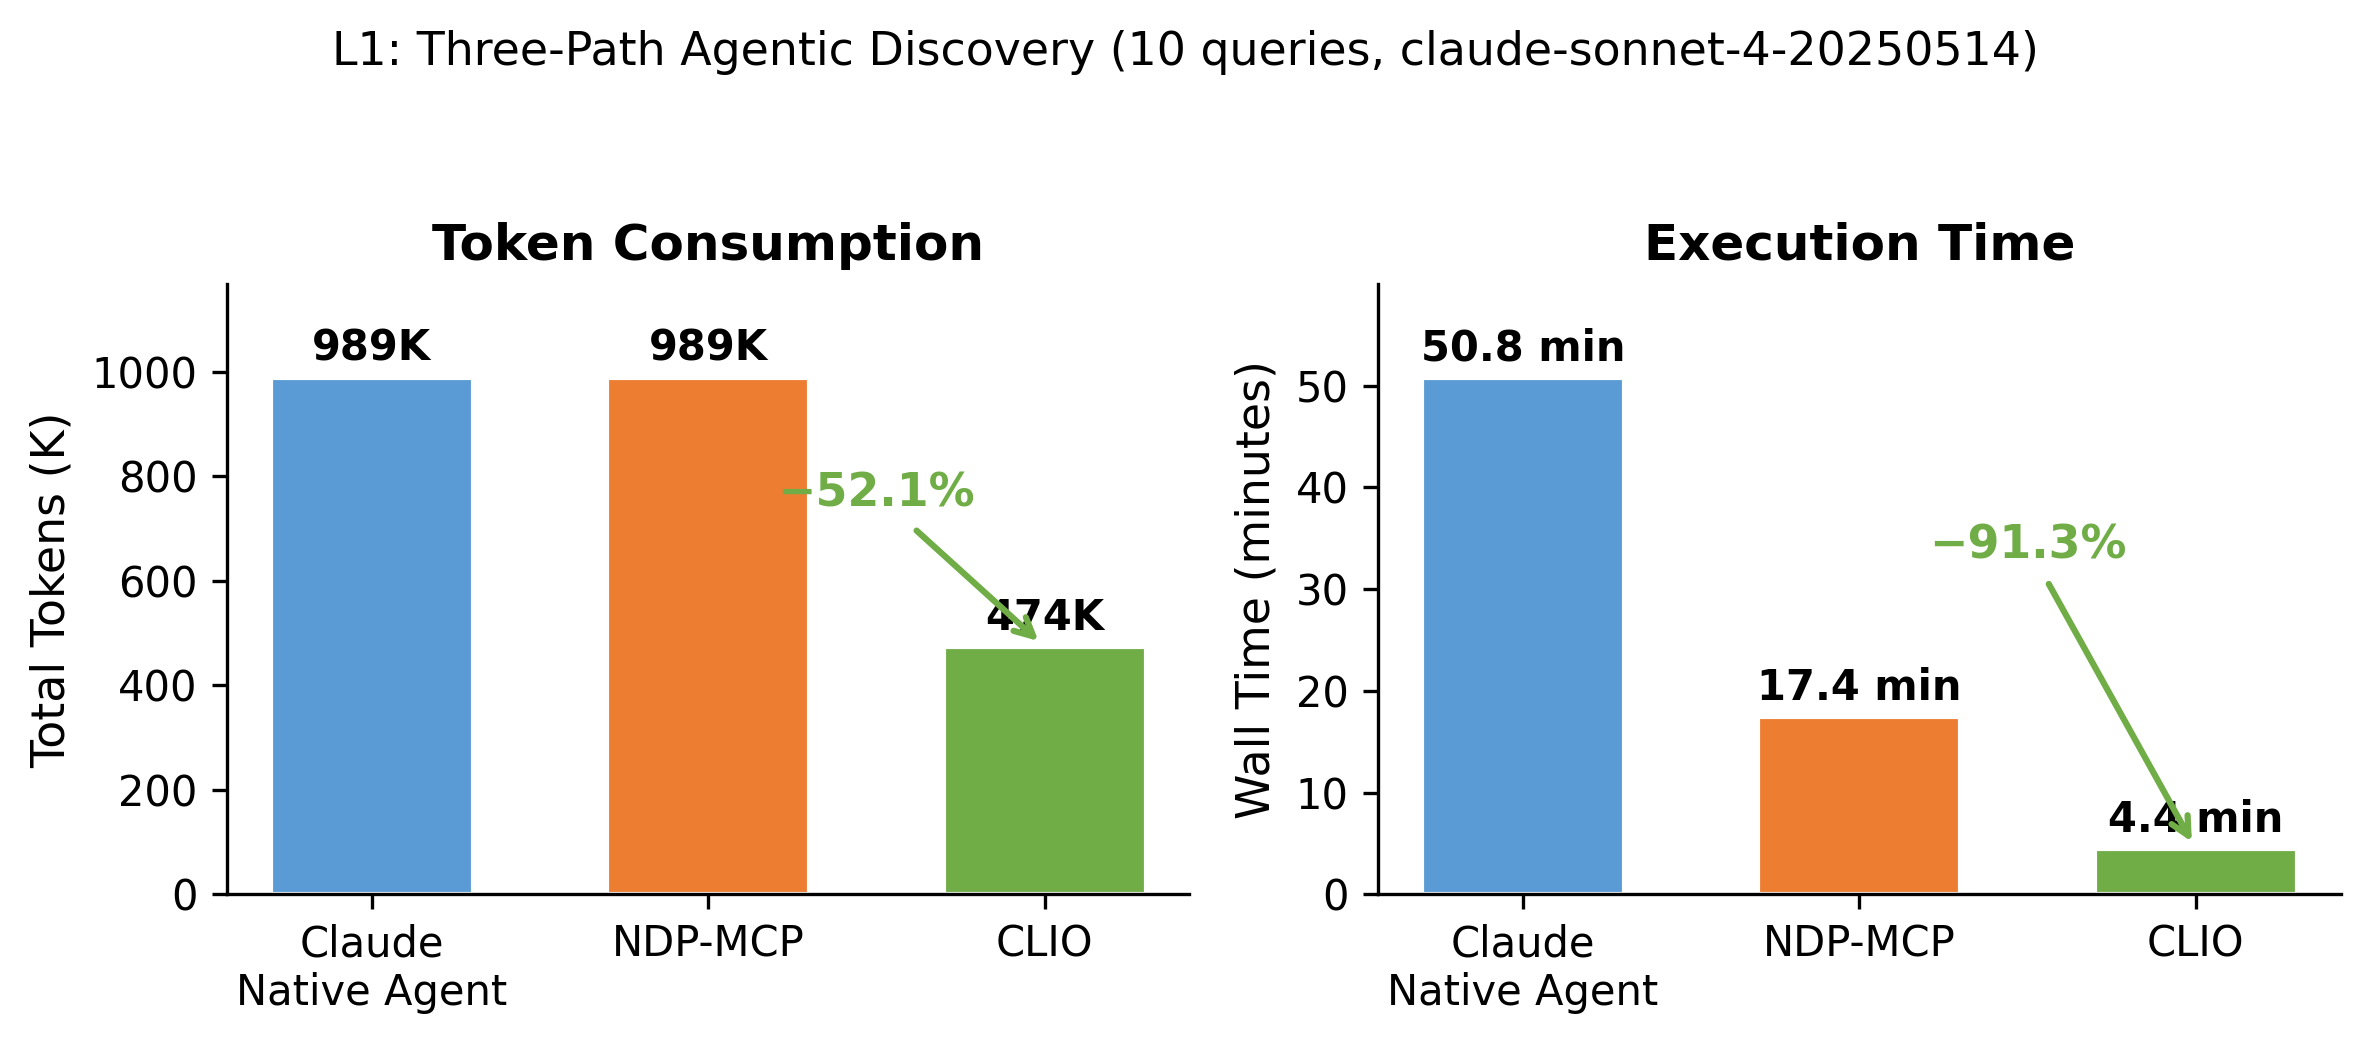
\includegraphics[width=0.85\columnwidth]{figures/fig_L1_three_path.png}
\caption{Agentic efficiency: total tokens (left) and wall time (right)
across 10~queries. CLIO achieves 52\% token and 91\% time reduction.}
\label{fig:l1-three-path}
\end{figure}

%% =====================================================================
\subsection{Science-Aware Retrieval Accuracy}
\label{sec:accuracy}

\textbf{Cross-unit retrieval.}
On 40~cross-unit queries (Table~\ref{tab:crossunit}), text baselines
cannot match across SI prefixes: a query for ``200~kPa'' never
lexically matches ``200000~Pa.'' BM25 achieves P@5 of 0.40; our
pipeline canonicalizes to SI base units at index time and achieves
\textbf{P@5 of 0.99} (+0.59 absolute) on the controlled benchmark.
On same-unit controls, all methods score within 0.05 P@5, confirming
gains are specific to cross-unit matching. R@5 is low across all
methods (0.07--0.19) because the 210-document corpus produces
approximately 42 relevant documents per query on average, making
recall at $K{=}5$ structurally bounded.

\begin{table}[!t]
\centering
\caption{Cross-unit retrieval at $K{=}5$ on controlled benchmark.}
\label{tab:crossunit}
\small
\renewcommand{\arraystretch}{1.2}
\begin{tabular}{l c c c c}
\toprule
\textbf{Method} & \textbf{P@5} & \textbf{R@5} & \textbf{F1@5} & \textbf{MRR} \\
\midrule
BM25-only          & 0.40 & 0.07 & 0.11 & 0.45 \\
\rowcolor{gray!5}
Dense-only         & 0.36 & 0.05 & 0.08 & 0.50 \\
Hybrid             & 0.36 & 0.07 & 0.10 & 0.47 \\
\rowcolor{gray!5}
String norm.       & 0.32 & 0.04 & 0.07 & 0.39 \\
\midrule
\rowcolor{gray!15}
\textbf{CLIO}      & \textbf{0.99} & \textbf{0.19} & \textbf{0.29} & \textbf{0.99} \\
\bottomrule
\end{tabular}
\renewcommand{\arraystretch}{1.15}
\end{table}

\begin{figure}[!t]
\centering
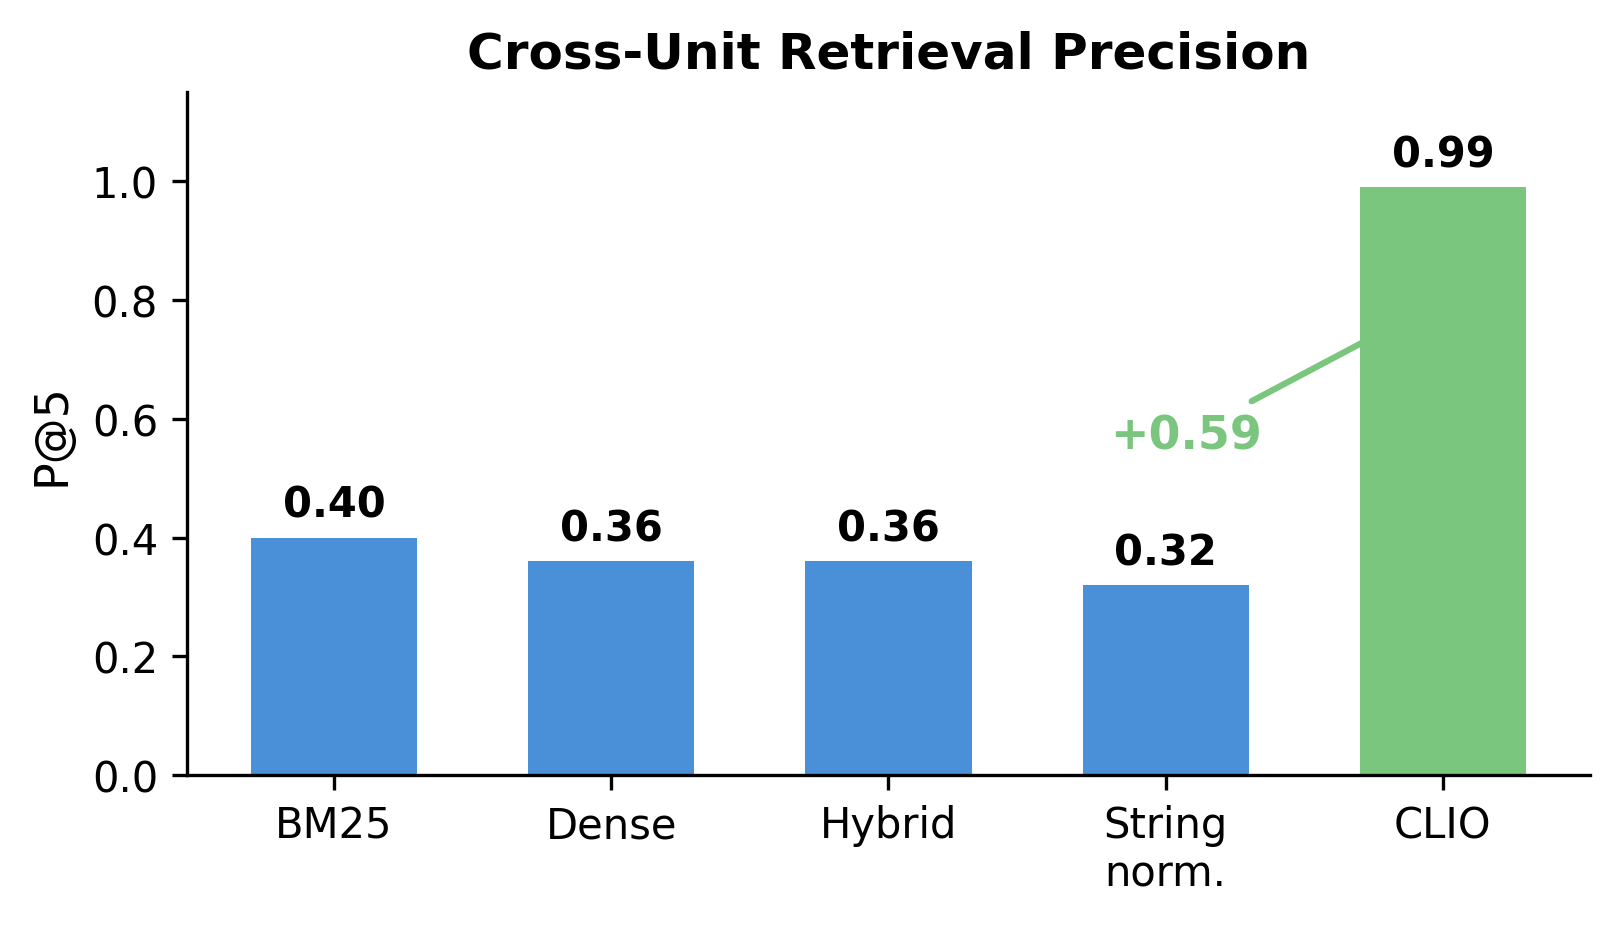
\includegraphics[width=0.85\columnwidth]{figures/fig_crossunit_p5_bar.png}
\caption{Cross-unit retrieval P@5. CLIO's science-aware operators achieve 0.99 vs.\ 0.40 for the best text baseline (+0.59 absolute).}
\label{fig:crossunit}
\end{figure}

\textbf{Baseline scope.} We compare against text-based retrieval
methods (BM25, dense, hybrid, string normalization) rather than
learned quantity-aware models (CONE, NC-Retriever, DeepQuant) because
(1)~these systems are not publicly reproducible on our benchmark,
and (2)~the comparison would be structurally unfair in both directions:
learned models achieve at best 0.54 binary accuracy on numerical
content~\cite{numeracygap2026} and 16.3\% on numeric
constraints~\cite{ncretriever2025}, while our benchmark is specifically
designed for cross-unit matching where arithmetic is required, not
approximated. The same-unit controls (P@5 0.30--0.45 across all
methods) confirm that our benchmark does not inflate scores through
general retrieval advantages.

\textbf{Real-world validation.} On 288~NOAA GHCN-Daily
documents~\cite{ghcn2012} (metric units only, queries in imperial),
CLIO achieves \textbf{0.700~P@5 (+87\%)} over the hybrid baseline
(0.375). No text method can match ``86\textdegree F'' against
``30.0~degC'' without arithmetic conversion
(Table~\ref{tab:real_world}).

\begin{table}[!t]
\centering
\caption{Real-world NOAA GHCN-Daily (288~docs, imperial queries).}
\label{tab:real_world}
\small
\begin{tabular}{lcccc}
\toprule
\textbf{Method} & \textbf{P@5} & \textbf{R@5} & \textbf{P@10} & \textbf{MRR} \\
\midrule
BM25            & 0.375 & 0.018 & 0.388 & 0.562 \\
\rowcolor{gray!5}
Hybrid          & 0.375 & 0.021 & 0.388 & 0.708 \\
\rowcolor{gray!15}
\textbf{CLIO}   & \textbf{0.700} & \textbf{0.055} & \textbf{0.725} & \textbf{0.760} \\
\bottomrule
\end{tabular}
\end{table}

\textbf{Formula matching (preliminary).} On 10~formula queries, BM25
achieves R@5 of 0.48 via loose text matching; CLIO achieves R@5 of
0.10 via strict symbolic equivalence. CLIO's formula operator requires
exact structural equivalence after canonicalization, producing fewer
but more reliable matches. We include formula normalization as a
proof-of-concept for combining symbolic and numeric operators in a
single retrieval pipeline; improving recall without sacrificing
precision is future work.

\textbf{Ablation.} Adding science operators (B$\to$C in
Table~\ref{tab:ablation}) produces the dominant gain: P@5 jumps from
0.36 to 0.99 (+0.63). The full pipeline (D) adds no further gain on
this benchmark, confirming that cross-unit matching is the bottleneck.
A no-LLM fallback achieves 96\% of LLM-assisted P@5, confirming that
the operators, not the language model, drive gains.

\begin{table}[!t]
\centering
\caption{Ablation: cumulative component contributions on cross-unit queries.}
\label{tab:ablation}
\small
\renewcommand{\arraystretch}{1.2}
\begin{tabular}{l l c c}
\toprule
 & \textbf{Components} & \textbf{P@5} & \textbf{MRR} \\
\midrule
A & Lexical (BM25)             & 0.40 & 0.45 \\
\rowcolor{gray!5}
B & A + dense vectors          & 0.36 & 0.47 \\
\rowcolor{gray!15}
\textbf{C} & \textbf{B + science operators} & \textbf{0.99} & \textbf{0.99} \\
\rowcolor{gray!5}
D & Full pipeline              & 0.99 & 0.99 \\
\bottomrule
\end{tabular}
\renewcommand{\arraystretch}{1.15}
\end{table}

\textbf{Metadata-adaptive strategy.} CLIO correctly classifies three
corpus variants (rich 87.5\% density $\to$ scientific branch, sparse
10.3\% $\to$ lexical+vector, no-metadata 4.4\% $\to$ lexical only)
and activates unit conversion only when extractable measurements exist.
We validate this on IOWarp blobs at scale: a rich-metadata variant
(2.5 measurements/blob) achieves 0.01\% inspection rate at 500K blobs
on DeltaAI GH200 with profiling at 90\,ms; a sparse variant
(0.75 measurements/blob) achieves 0.05\% at 100K with profiling at
47\,ms. CLIO adapts its strategy per variant while maintaining
cross-unit correctness.
To evaluate federated search, we index 100~namespaces (30~rich-scientific, 30~sparse, 30~pure-text, 5~formula, 5~empty) and issue cross-unit queries. Corpus profiling achieves \textbf{routing recall of 1.0} (zero false negatives) while skipping 52\% of namespaces that lack scientific metadata at 9\,ms per namespace, reducing search cost by 52\% with no recall loss.

%% =====================================================================
\subsection{Storage Integration and Scaling}
\label{sec:storage-scaling}

\textbf{IOWarp blob storage.}
IOWarp's Context Transfer Engine (Sec.~3.1) organizes scientific data
as blobs grouped under tags across tiered storage. Its native
BlobQuery API returns all blobs matching a tag regex with no content
filtering. CLIO
addresses this by indexing scientific metadata from blobs at ingest
time. We store synthetic scientific blobs across four tags
(temperature in \textdegree C, pressure in kPa, wind in m/s) and
issue four cross-unit queries using mismatched units
(\textdegree F, psi, km/h). Table~\ref{tab:iowarp} reports results
on DeltaAI GH200 nodes (in-memory path) and Docker (CTE-backed path);
both produce identical cross-unit results.

\begin{table}[t]
\centering
\caption{CLIO on IOWarp blobs (DeltaAI GH200). Rich = 2.5~meas/blob,
Sparse = 0.75~meas/blob. CLIO returns top-50 unit-converted matches;
BlobQuery returns all blobs unfiltered.}
\label{tab:iowarp}
\footnotesize
\setlength{\tabcolsep}{3pt}
\begin{tabular}{@{}r r r r r r@{}}
\toprule
\textbf{Blobs} & \textbf{Index} & \textbf{Profile} & \textbf{Meas.} & \textbf{CLIO} & \textbf{BlobQ.} \\
\midrule
\multicolumn{6}{@{}l}{\textit{Rich metadata (2.5 measurements per blob)}} \\
1K   & 163\,s     & 17\,ms & 2{,}500   & 50 & 250 \\
10K  & 822\,s     & 27\,ms & 25{,}000  & 50 & 2{,}500 \\
50K  & 4{,}718\,s & 45\,ms & 125{,}000 & 50 & 12{,}500 \\
100K & 9{,}801\,s & 51\,ms & 250{,}000 & 50 & 25{,}000 \\
500K & 56{,}215\,s & 90\,ms & 1{,}250{,}000 & 50 & 125{,}000 \\
\midrule
\multicolumn{6}{@{}l}{\textit{Sparse metadata (0.75 measurements per blob)}} \\
1K   &  58\,s     & 11\,ms &    750    & 50 & 250 \\
10K  & 702\,s     & 33\,ms &  7{,}500  & 50 & 2{,}500 \\
50K  & 3{,}852\,s & 41\,ms &  37{,}500 & 50 & 12{,}500 \\
100K & 8{,}068\,s & 47\,ms &  75{,}000 & 50 & 25{,}000 \\
\rowcolor{red!10}
500K & \multicolumn{5}{c}{\textit{pending}} \\
\bottomrule
\end{tabular}
\end{table}

CLIO finds cross-unit matches at every scale while BlobQuery cannot
filter by content (Table~\ref{tab:iowarp}, Fig.~\ref{fig:iowarp-scaling}). The inspection rate falls
from 5.0\% at 1K to \textbf{0.01\% at 500K} ($5{,}000\times$ reduction
over BlobQuery). Corpus profiling scales sub-linearly: 500$\times$
data growth (1K to 500K) produces only $5.3\times$ profiling increase
(17\,ms to 90\,ms on GH200).

\begin{figure}[t]
\centering
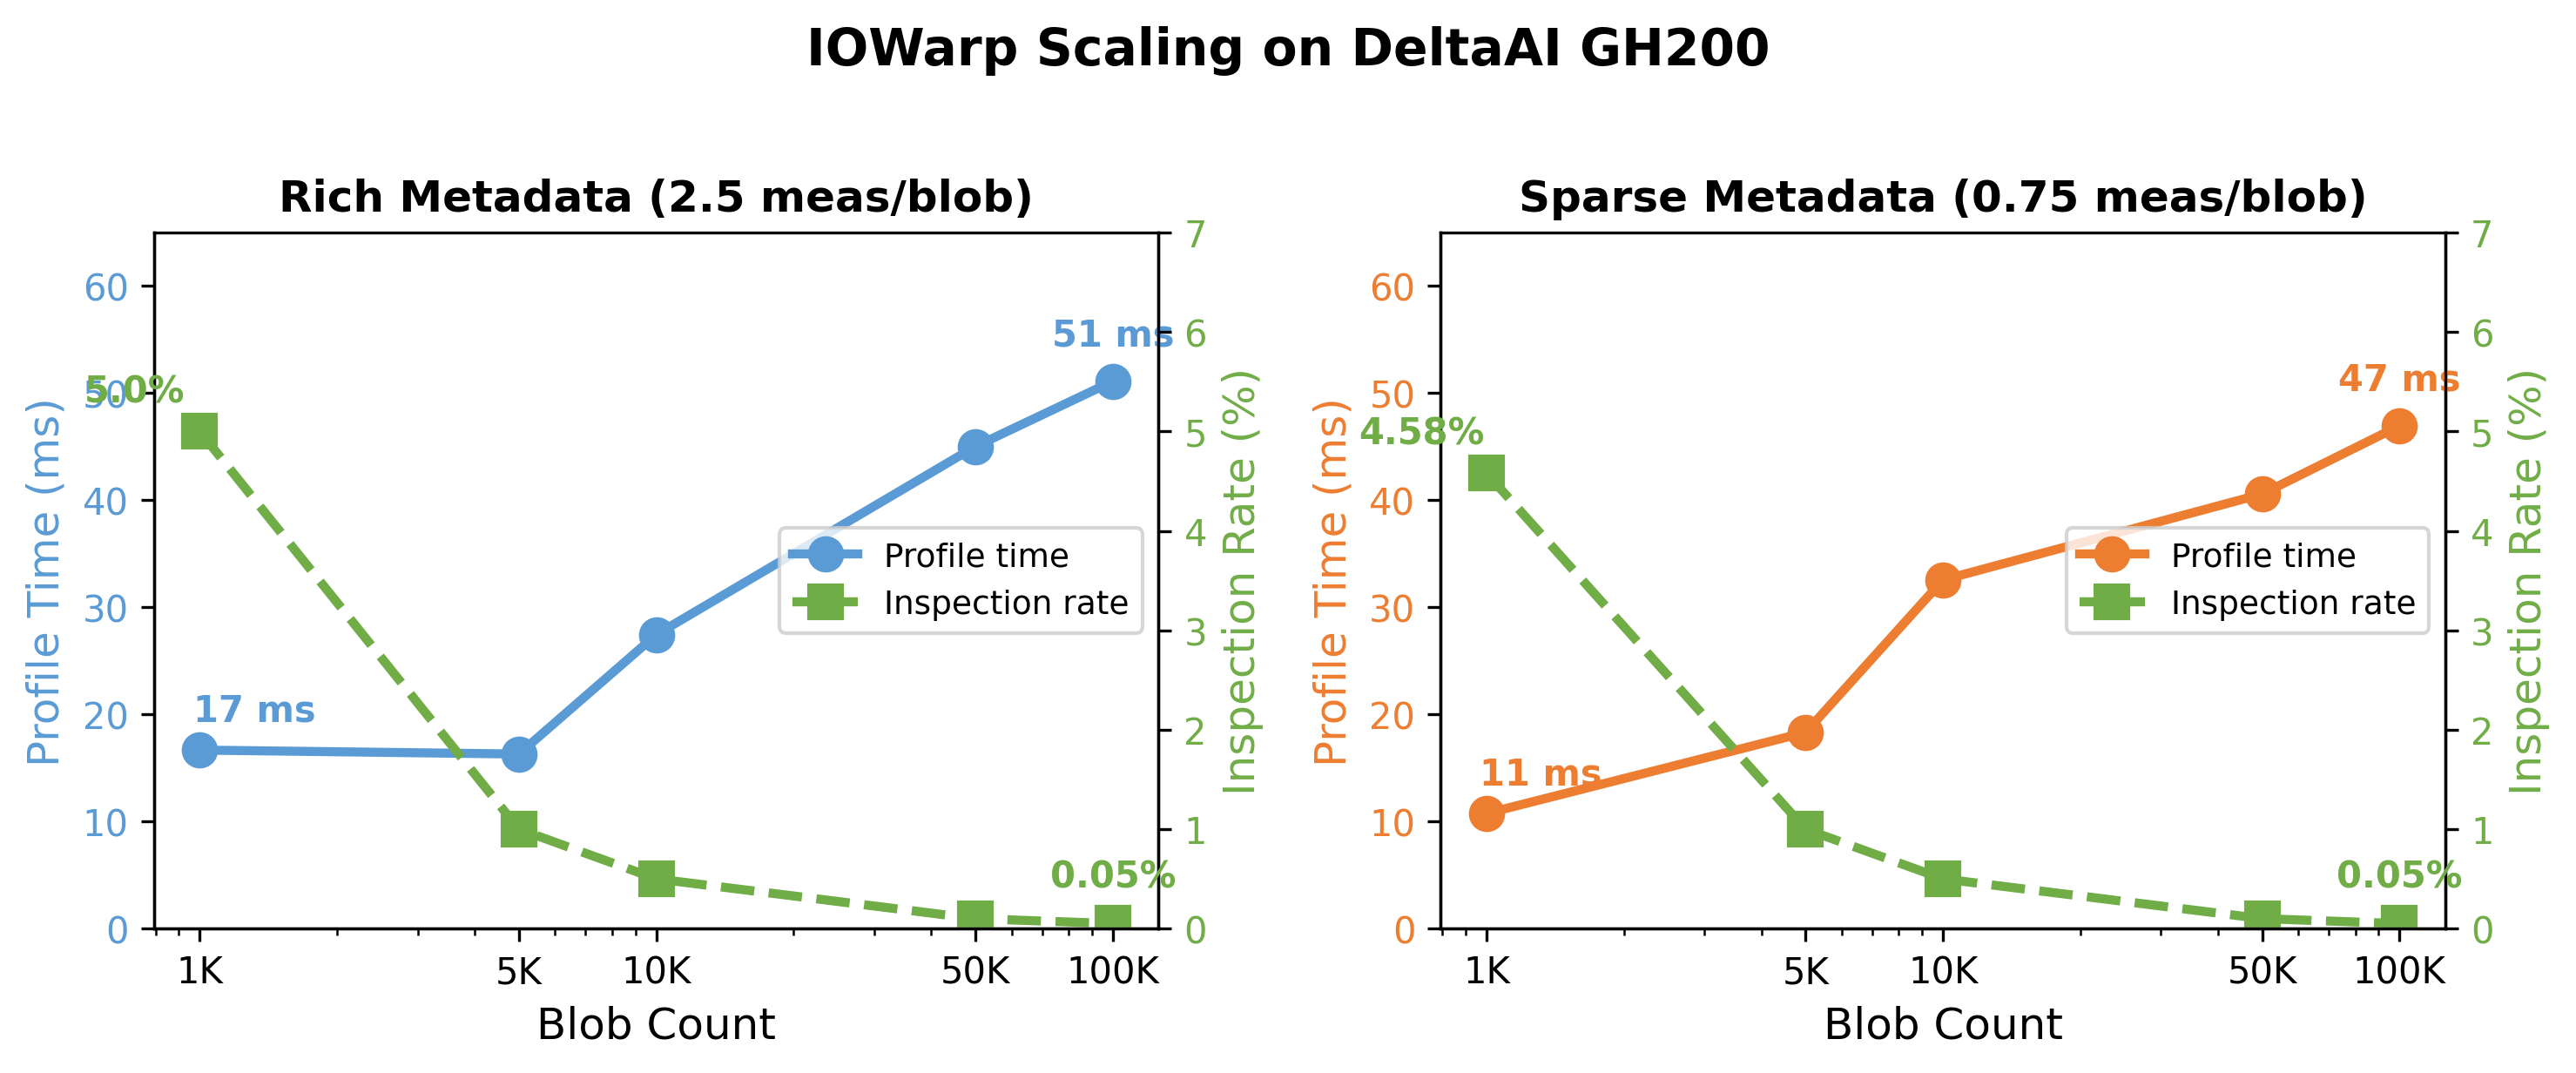
\includegraphics[width=\columnwidth]{figures/fig_iowarp_scaling.png}
\caption{IOWarp scaling on DeltaAI GH200: profiling time (left) and
inspection rate (right). Rich metadata: 1K--500K blobs; sparse
metadata: 1K--100K (500K pending). Inspection drops to 0.01\% at 500K
for rich metadata.}
\label{fig:iowarp-scaling}
\end{figure}

\textbf{Distributed scaling on 2.5M arXiv abstracts.}
We evaluate CLIO's coordinator--worker pipeline on NCSA DeltaAI
(GH200 nodes) with 2.5M arXiv abstracts across four DuckDB shards
(625K each). 80~queries per configuration.

\begin{table}[t]
\centering
\caption{Query latency (ms) on DeltaAI GH200. Strong scaling holds the
2.5M corpus fixed; weak scaling grows data with workers.}
\label{tab:scaling}
\small
\begin{tabular}{l r r r r r}
\toprule
& \textbf{Workers} & \textbf{Corpus} & \textbf{p50} & \textbf{p95} & \textbf{Eff.} \\
\midrule
\multirow{3}{*}{\rotatebox{90}{\footnotesize Strong}}
& 1 & 2.5M & 39.0 & 41.5 & --- \\
& 2 & 2.5M & 40.7 & 43.7 & --- \\
& 4 & 2.5M & 41.6 & 62.1 & --- \\
\midrule
\multirow{3}{*}{\rotatebox{90}{\footnotesize Weak}}
& 1 & 625K  & 38.5 & 41.2 & 1.00 \\
& 2 & 1.25M & 39.4 & 42.1 & 0.98 \\
& 4 & 2.5M  & 41.0 & 59.0 & 0.94 \\
\bottomrule
\end{tabular}
\end{table}

All queries complete under 70\,ms with p50 under 42\,ms across
2.5M~documents (Table~\ref{tab:scaling}). Weak scaling efficiency
reaches \textbf{0.94} at $4\times$ scale, demonstrating that CLIO's
architecture supports horizontal scale-out with minimal coordinator
overhead.

\textbf{Cross-unit correctness at distributed scale.}
To verify that dimensional conversion remains correct when the corpus
is distributed, we issue cross-unit probe queries against the 70K-document
distributed corpus (4~shards on DeltaAI GH200). Fig.~\ref{fig:d4-correctness}
shows that querying in different units yields \emph{identical hit counts}:
100~kPa, 100{,}000~Pa, 1~bar, and 0.987~atm all return exactly 12~hits;
30\textdegree C, 86\textdegree F, and 303.15~K all return exactly
20~hits at sub-50\,ms latency. This confirms that SI canonicalization
is consistent across shards.

\begin{figure}[t]
\centering
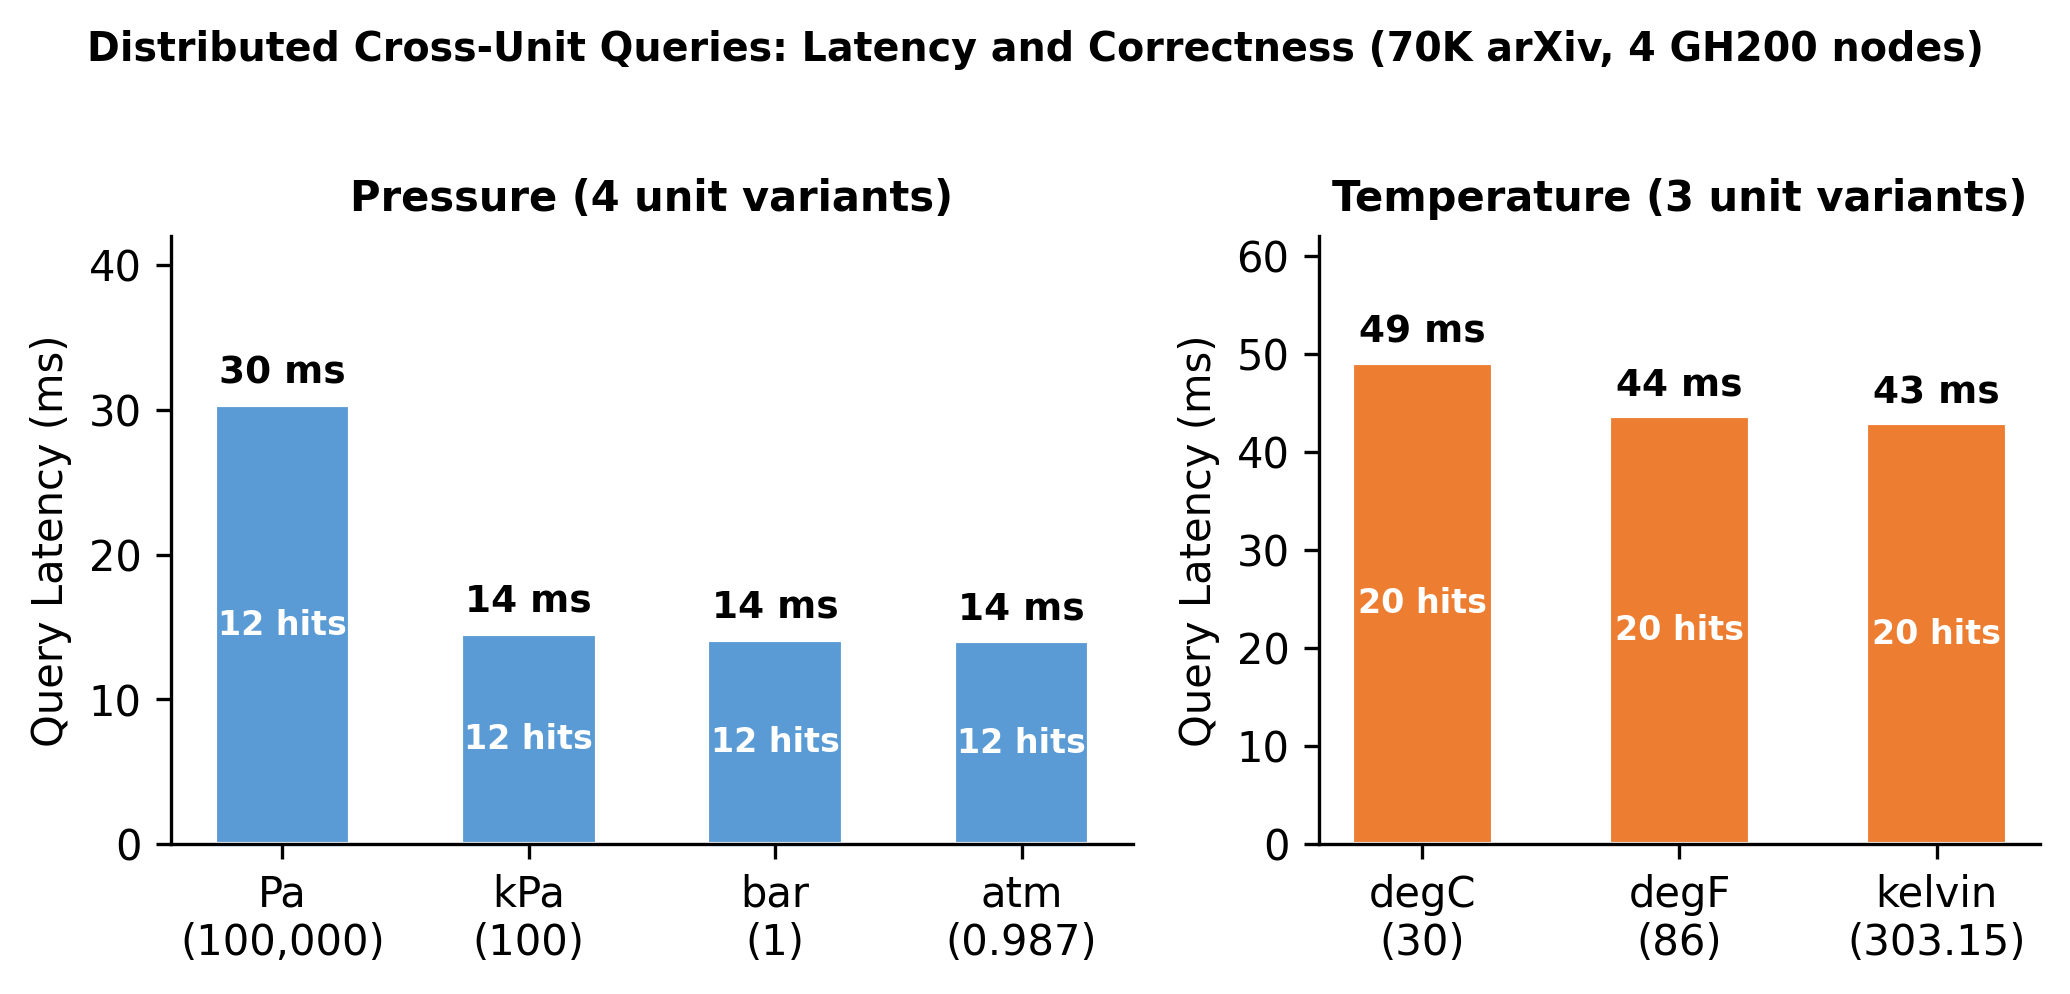
\includegraphics[width=\columnwidth]{figures/fig_d4_crossunit_correctness.png}
\caption{Distributed cross-unit queries on 70K arXiv (4~GH200 nodes).
All unit variants return identical hit counts (correctness) at
sub-50\,ms latency. Pa is slower than kPa/bar/atm due to larger
raw-value range scan.}
\label{fig:d4-correctness}
\end{figure}

\textbf{Numeric query coverage at scale.}
We run 20~scientific numeric queries spanning 16~unit types (GeV, nm,
GHz, kelvin, kPa, tesla, etc.) against the distributed corpus. All
20~queries return results (\textbf{100\% hit rate}) with p50 latency
of 42\,ms and p99 of 62\,ms, demonstrating that CLIO's unit registry
generalizes beyond the controlled benchmark to real scientific
literature at scale.

\textbf{Limitations.} The regex extractor misses non-standard formats
(``$2 \times 10^3$~Pa''), achieving 95\% precision / 90\% recall;
missed measurements fall through to lexical and vector branches
rather than causing silent omission.
Compound units (N/m$^2$, mol/L) are unsupported and fall back to
lexical retrieval. The 58-unit registry (12~SI domains) is extensible
by adding rows without code changes.
Scaling beyond 4~GH200 nodes and 2.5M documents remains future work.
The controlled benchmark is synthetic; the NOAA evaluation
(288~real documents) partially addresses ecological validity.

%% ===================================================================
%% Section 6: Conclusion
